\documentclass[a4paper,11pt]{article}

\usepackage[french]{babel}
\usepackage[T1]{fontenc}
\usepackage[utf8]{inputenc}
\usepackage{graphicx}
%\usepackage{fullpage}

\begin{document}

\title{\textbf{Compte rendu du TP \no 5}\\Segmentation d’une image par Split and Merge}
\author{Thibaut Castanié\\\textit{Master IMAGINA}}
\date{\today}

\maketitle
\thispagestyle{empty}

\newpage 
\section{Division d'une image en 4 régions}
L'image utilisée pour la suite du TP est la suivante :
\begin{center}

\includegraphics[scale=0.6]{rollo.png}\\
\textit{L'image originale rollo.ppm}
\end{center}

\paragraph{Méthodologie utilisée} Pour diviser une image en 4 régions de taille égales, j'ai utilisé le schéma suivant afin de nommer les zones obtenues. Cette numérotation sera utilisée de la même manière tout le long du TP.
\begin{center}
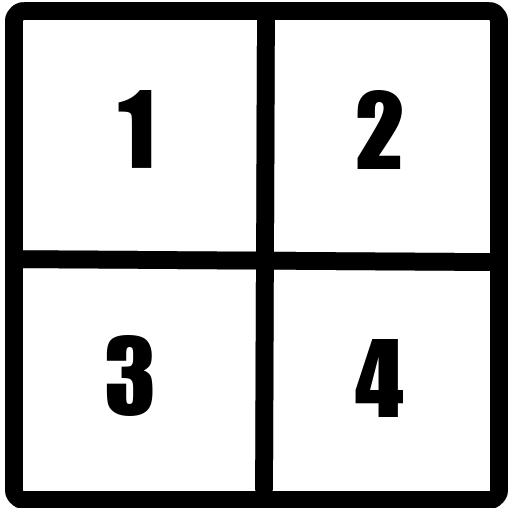
\includegraphics[scale=0.25]{schema.png}\\
\textit{Schématisation de la division d'une image}
\end{center}

\paragraph{Division de l'image} L'image originale est divisée en quatre parties égales, et chaque partie est de la couleur de la moyenne des couleurs des pixels la composant.
\begin{center}

\includegraphics[scale=0.6]{rolloDivMoy.png}\\
\textit{L'image de sortie contenant les 4 valeurs moyennes}
\end{center}

\paragraph{Variance}
\begin{itemize}
\item Zone 1 : 16.4444
\item Zone 2 : 3516.71
\item Zone 3 : 4263.54
\item Zone 4 : 4474.51
\end{itemize}
En calculant la racine carrée de la variance, on obtient la valeur moyenne d'écart entre la moyenne calculée et la valeurs des pixels.

\newpage
\section{Etape de division récursive}
\begin{verbatim}
paramètres : imgEntree, imgSortie,
             coordonnées x et y du point haut-gauche,
             nbPixels, hauteur, largeur, seuil.
fonction divRecursive
    somme1, somme2, somme3, somme4 = 0.
    variance1, variance2, variance3, variance4 = 0.
    pour chaque pixel de (x,y) à (x+hauteur,y+largeur)
        si le pixel est dans le premier quart
            on ajoute sa valeur dans somme1
        si le pixel est dans le second quart
            on ajoute sa valeur dans somme2
        si le pixel est dans le troisème quart
            on ajoute sa valeur dans somme3
        si le pixel est dans le quatrième quart
            on ajoute sa valeur dans somme4
    pour i de 1 à 4
        moyenne(i) = somme(i) / (nbPixels/4)
        dessinerCarré sur le ième quart de couleur moyenne(i)
    pour chaque pixel de (x,y) à (x+hauteur,y+largeur)
        si le pixel est dans le premier quart
            on ajoute (valeur du Pixel - moyenne1)^2  dans variance1
        si le pixel est dans le second quart
            on ajoute (valeur du Pixel - moyenne2)^2  dans variance2
        si le pixel est dans le troisème quart
            on ajoute (valeur du Pixel - moyenne3)^2  dans variance3
        si le pixel est dans le quatrième quart
            on ajoute (valeur du Pixel - moyenne4)^2  dans variance4
    pour i de 1 à 4
        variance(i) = variance(i) /4.
    si racine carrée de variance1 > seuil
        divRecursive(imgEntree, imgSortie,x,y,
                     nbPixels/4,hauteur/2,largeur/2,seuil)
    si racine carrée de variance2 > seuil
        divRecursive(imgEntree, imgSortie,x,y+(largeur/2),
                     nbPixels/4,hauteur/2,largeur/2,seuil)
    si racine carrée de variance3 > seuil
        divRecursive(imgEntree, imgSortie,x+(hauteur/2),y,
                     nbPixels/4,hauteur/2,largeur/2,seuil)
    si racine carrée de variance4 > seuil
        divRecursive(imgEntree, imgSortie,x+(hauteur/2),y+(largeur/2),
                     nbPixels/4,hauteur/2,largeur/2,seuil)
fin;
\end{verbatim}
\paragraph{Images divisées récursivement}
\vspace{2cm}
\begin{center}

\includegraphics[scale=0.33]{rolloRec40.png}
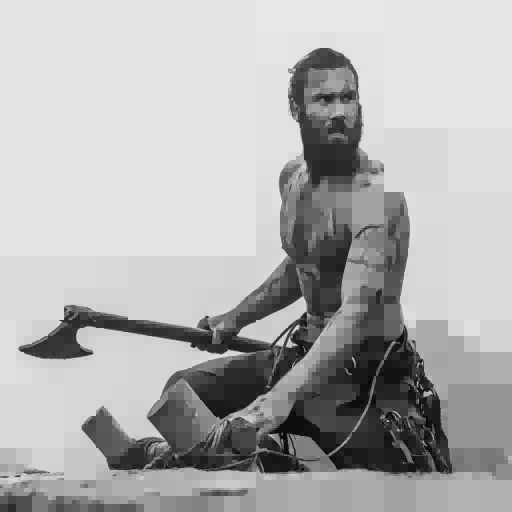
\includegraphics[scale=0.33]{rolloRec20.png}\\

\includegraphics[scale=0.33]{rolloRec10.png}

\includegraphics[scale=0.33]{rolloRec05.png}\\
\textit{L'image divisée avec un seuil de 40, 20, 10 puis 5}
\end{center}


\newpage
\section{Etape de fusion}
\begin{center}
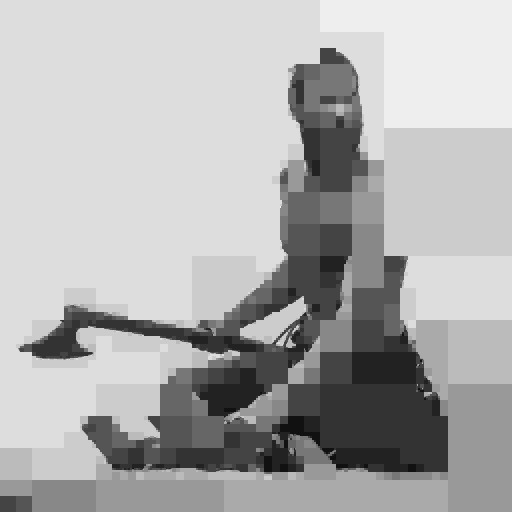
\includegraphics[scale=0.6]{rolloRecTraf.png}
\end{center}

\end{document}